\chapter{Theoretical Background}

This chapter establishes the theoretical and mathematical foundations required to contextualize the contributions of this document. It provides a critical review of the current literature surrounding neuroevolutionary algorithms, Spiking Neural Networks (SNNs), and biologically plausible learning rules. By analyzing recent advancements and their inherent limitations, this section constructs the conceptual framework necessary to justify the proposed Spiking-NEAT architecture and its application in dynamic control environments.





\section{Neuroevolution and Genetic Algorithms}

Historically, the standard method for training Artificial Neural Networks (ANNs) is the backpropagation algorithm. The fundamental purpose of backpropagation is to optimize a network's predictions through supervised learning by systematically adjusting its internal weights and biases to minimize a mathematical error \cite{mnih2015human}.

\begin{figure}[htbp]
    \centering
    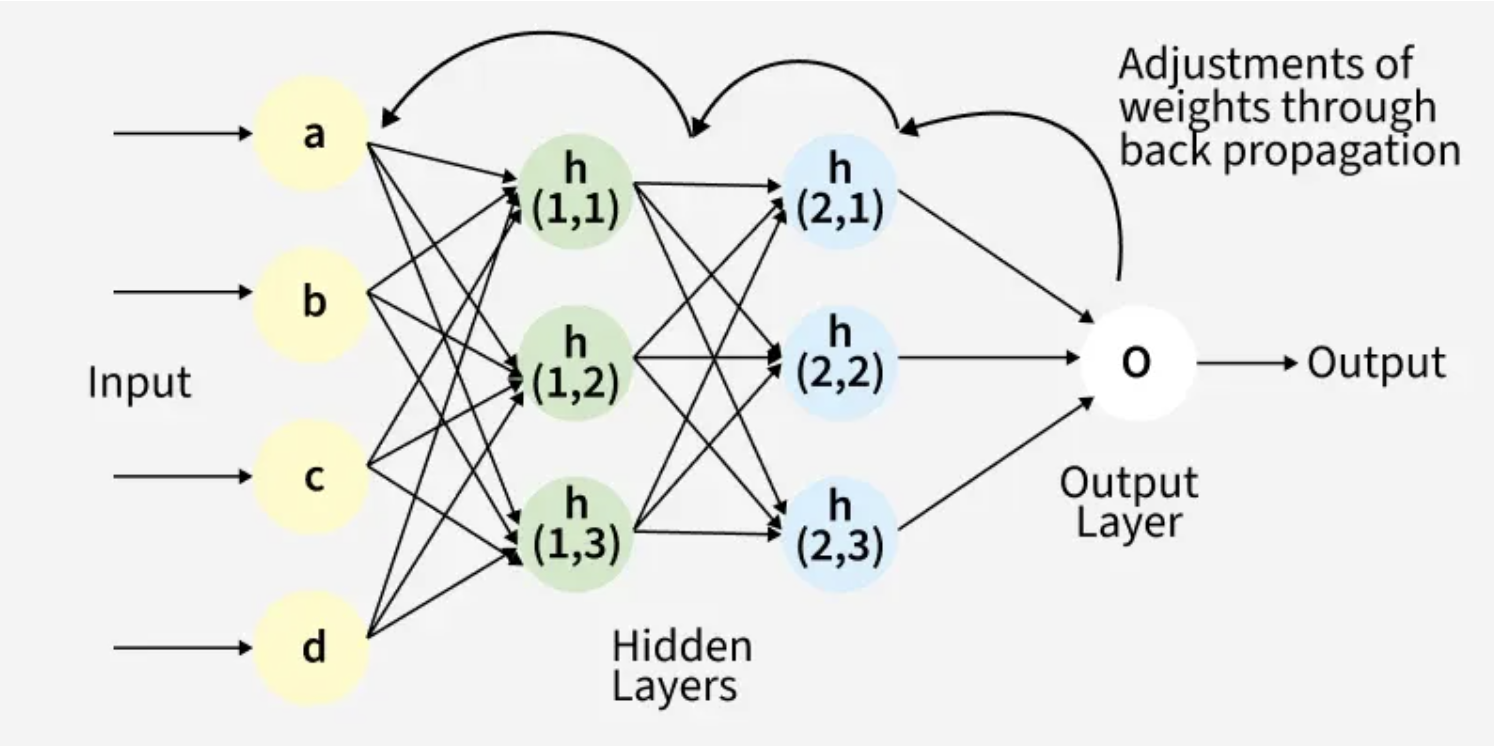
\includegraphics[width=0.85\textwidth]{imaxes/backpropagation.png}
    \caption{Architecture of a feedforward neural network illustrating the forward pass of activations and the backward propagation of error adjustments for weight optimization. Adapted from GeeksforGeeks.}
    \label{fig:backpropagation}
\end{figure}

As illustrated in Figure~\ref{fig:backpropagation}, this training process operates in four distinct phases:

\begin{enumerate}
    \item \textbf{The Forward Pass:} Input data propagates forward through the network's interconnected hidden layers. Each node extracts features and applies continuous mathematical transformations until the final layer outputs a prediction.
    \item \textbf{Error Calculation:} A predefined loss function evaluates this output, measuring the mathematical discrepancy (the error) between the network's prediction and the actual ``ground truth'' provided by the training dataset.
    \item \textbf{The Backward Pass:} The algorithm calculates the gradient of the loss function. It then moves backward through the network, effectively distributing the ``blame'' for the error by calculating exactly how much each individual weight and bias needs to be adjusted to improve the next prediction.
    \item \textbf{The Optimizer Step:} An optimizer uses the calculated gradients to update the network weights and improve the next prediction.
\end{enumerate}

While this gradient descent method is incredibly powerful for supervised tasks like image classification, it possesses two strict requirements: it relies on massive datasets of ``correct answers'' to calculate the initial loss, and it requires continuous, differentiable activation functions to calculate the gradients.

However, in dynamic control environments (such as autonomous robotics or video games like Super Mario Bros) there is no dataset of ``perfect moves'' to learn from. The AI only knows whether it survived or failed based on sparse environmental rewards. Because standard gradient-based backpropagation struggles in these unpredictable, data-poor scenarios, researchers turned to biology for a solution, giving rise to Neuroevolution (NE).

Neuroevolution is a prominent subfield of Artificial Intelligence that applies the principles of Darwinian natural selection to neural networks. Instead of training a single network with a dataset, Neuroevolution relies on Genetic Algorithms (GAs) to generate a "population" of many different candidate networks. The algorithm evaluates each network based on its performance in the environment (its fitness). The weakest networks are discarded, while the most successful ones are selected to produce a new generation through biological mechanics like crossover (combining traits from two parents) and mutation (random structural changes).

\subsection{TWEANNs}

Historically, early neuroevolutionary systems focused exclusively on optimizing the synaptic weights of a neural network, while its structural topology remained fixed by a human engineer. However, guessing the optimal architecture for a complex, dynamic environment is incredibly difficult. To overcome this, researchers developed Topology and Weight Evolving Artificial Neural Networks (TWEANNs) \cite{stanley2002}, algorithms designed to evolve both the connection weights and the physical structure of the network simultaneously.

While TWEANNs represented a significant conceptual leap, their practical application was severely hindered by three critical limitations:

\begin{enumerate}
    \item \textbf{The Competing Conventions (Permutation) Problem:} This is the most severe flaw in early neuroevolution. It occurs when two parent networks learn to solve the same problem, but encode their solutions using different internal topological orderings. If a genetic algorithm attempts to cross over (breed) these two parents, the resulting offspring will often suffer from missing or duplicated features. Because the algorithm has no way to align the mismatched hidden nodes, crossing over two highly successful parents frequently produces damaged offspring.
\end{enumerate}

\begin{figure}[htbp]
    \centering
    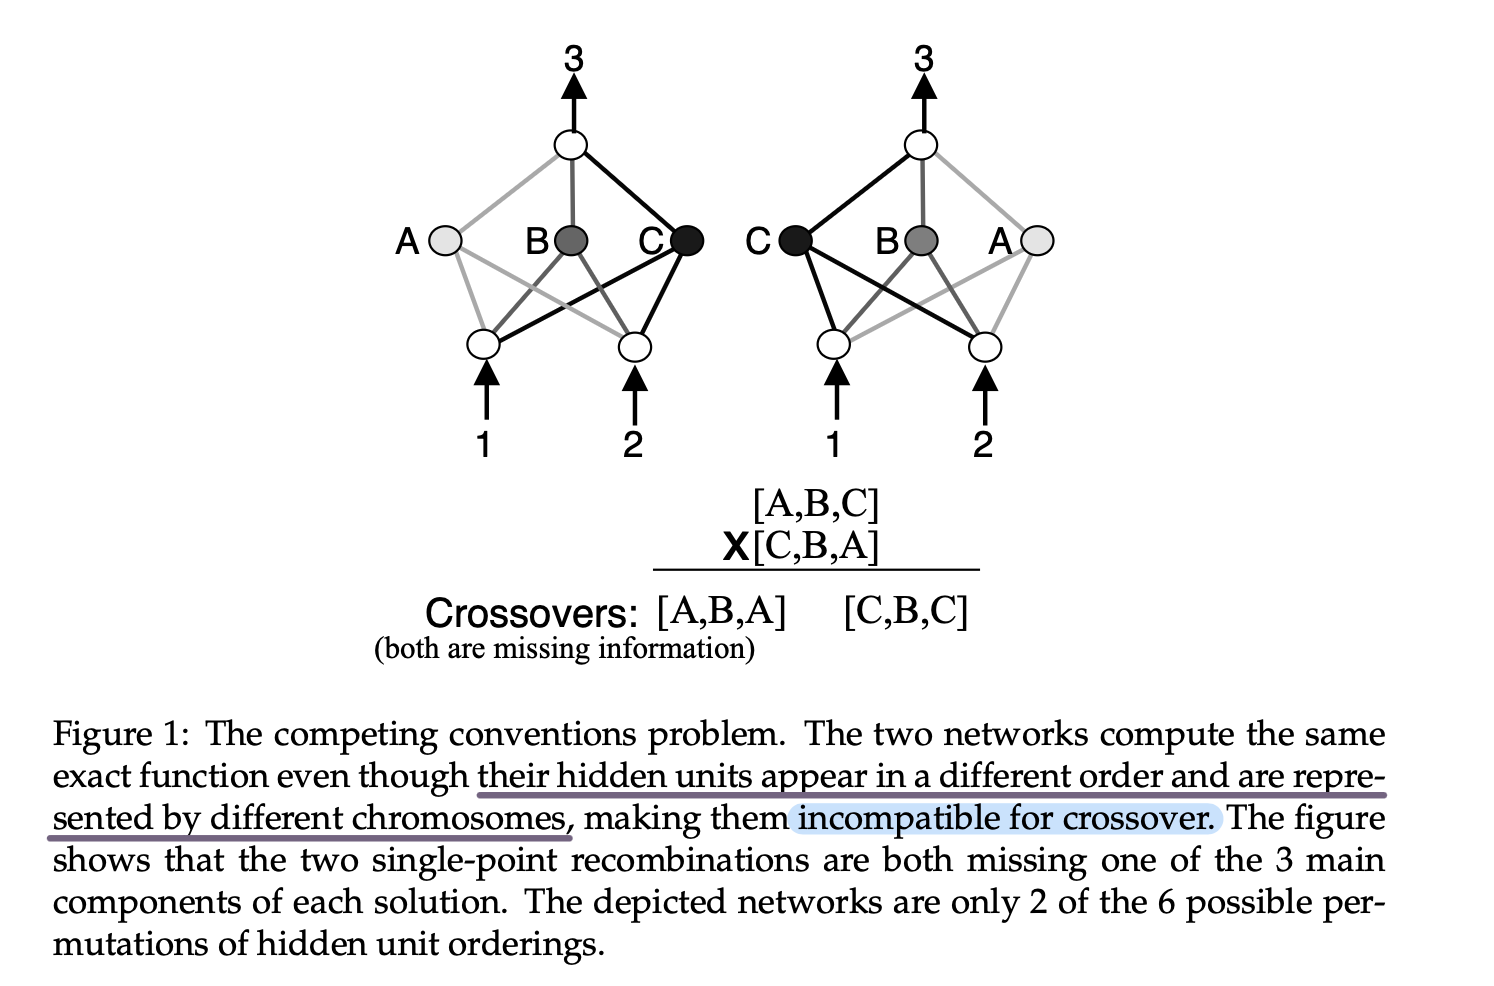
\includegraphics[width=0.85\textwidth]{imaxes/tweanns1.png}
    \caption{The competing conventions problem. The two networks compute the same exact function even though their hidden units appear in a different order and are represented by different chromosomes, making them incompatible for crossover. The figure shows that the two single-point recombinations are both missing one of the 3 main components of each solution. The depicted networks are only 2 of the 6 possible permutations of hidden unit orderings. Adapted from \cite{stanley2002}.}
    \label{fig:competing_conventions}
\end{figure}

As illustrated in Figure~\ref{fig:competing_conventions}, crossing over two functional networks with different internal orderings results in offspring missing crucial information (e.g., missing node C or node A).

\begin{figure}[htbp]
    \centering
    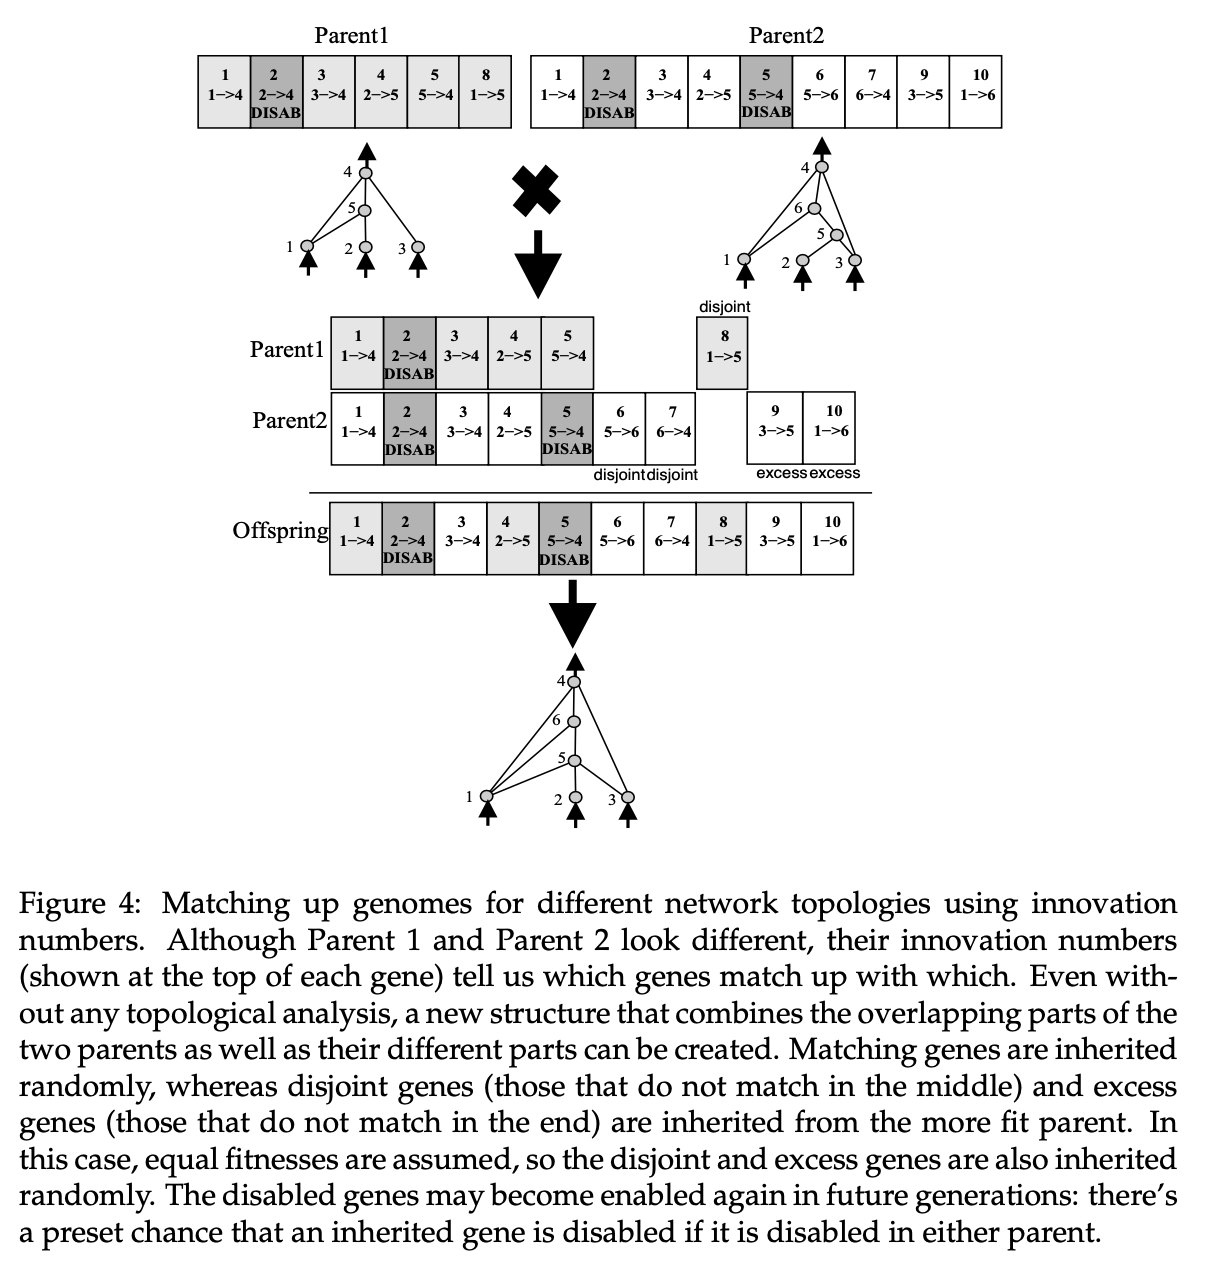
\includegraphics[width=0.9\textwidth]{imaxes/tweanns2.png}
    \caption{Matching up genomes for different network topologies using innovation numbers. Although Parent 1 and Parent 2 look different, their innovation numbers (shown at the top of each gene) tell us which genes match up with which. Even without any topological analysis, a new structure that combines the overlapping parts of the two parents as well as their different parts can be created. Matching genes are inherited randomly, whereas disjoint genes (those that do not match in the middle) and excess genes (those that do not match in the end) are inherited from the more fit parent. In this case, equal fitnesses are assumed, so the disjoint and excess genes are also inherited randomly. The disabled genes may become enabled again in future generations: there is a preset chance that an inherited gene is disabled if it is disabled in either parent. Adapted from \cite{stanley2002}.}
    \label{fig:innovation_numbers}
\end{figure}

\begin{enumerate}
    \setcounter{enumi}{1} % fuerza a que la lista empiece en el número 2
    \item \textbf{Unprotected Innovation:} In evolutionary algorithms, a newly mutated structure (like a new hidden node) often causes a temporary drop in performance before its weights can be optimized. Early TWEANNs evaluated all networks in a single, unified pool. Consequently, new and complex topological innovations were immediately driven to extinction by older, structurally simpler networks that had already optimized their weights. Also, having the global population all together can cause the initially ``stronger'' genes to prevail and drive other species of the global population to extinction; this is a hazard for innovation.
    
    \item \textbf{Topological Bloat:} To ensure genetic diversity, early models frequently initialized populations with complex, highly randomized topologies. This bloated the genomes with unjustified connections from the very first generation, unnecessarily expanding the mathematical search space and wasting computational resources.
\end{enumerate}

These three structural flaws meant that TWEANNs struggled to scale to high-dimensional tasks. The field required a paradigm shift to make neuroevolution mathematically efficient and viable for complex control environments, a shift that was realized by the introduction of the NEAT algorithm.


\subsection{NeuroEvolution of Augmented Topologies (NEAT)}

NeuroEvolution of Augmented Topologies (NEAT) \cite{stanley2002} is a highly effective algorithm that resolves the historical limitations of TWEANNs. As detailed by Stanley and Miikkulainen \cite{stanley2002}, NEAT achieves increased efficiency through a principled method of crossover via historical markings, protection of structural innovation using speciation, and incremental growth from minimal structures. These mechanisms allow evolution to optimize and complexify solutions simultaneously, providing a powerful foundation for dynamic control tasks.

\subsubsection{Innovation Numbers}
The fundamental mechanism that allows NEAT to resolve the Competing Conventions problem is the implementation of historical markings, or innovation numbers. In biological evolution, homology allows organisms with different genetic structures to cross over safely because their genes share a common historical origin. NEAT mathematically replicates this biological principle by assigning a unique, incrementally increasing integer, a global innovation number, to every new structural mutation (such as a new connection or a new hidden node) that occurs within the population.

This historical tracking transforms the complex topological analysis required by earlier TWEANNs into a highly efficient linear alignment problem. When two parent networks are selected for crossover, their genomes are aligned side-by-side using these numerical IDs. To perform this crossover without losing information, the algorithm categorizes the aligned genes into three distinct types:

\begin{itemize}
    \item \textbf{Matching genes:} Genes with the exact same innovation number present in both parents. These genes are inherited randomly by the offspring.
    \item \textbf{Disjoint genes:} Genes present in one parent but completely missing in the other. These genes do not match in the middle of the genome sequence.
    \item \textbf{Excess genes:} Genes present in one parent but missing in the other. These genes do not match at the end of the genome sequence, falling outside the numerical range of the overlapping innovation numbers.
\end{itemize}

During the recombination process, disjoint and excess genes are systematically inherited from the more fit parent to ensure advantageous structures are preserved. If both parents share equal fitness levels, these disjoint and excess genes are instead inherited randomly. Furthermore, to preserve structural memory, there is a preset probability that an inherited gene will remain disabled in the offspring if it was disabled in either of the parent genomes.

By utilizing these historical markings, NEAT guarantees that crossover remains orderly. The algorithm can seamlessly recombine networks of vastly different sizes and topologies without losing track of which gene performs which function, effectively ensuring that structural innovations are safely transferred to the next generation without information loss.

\subsubsection{Speciation}
The second major mechanism NEAT introduces to stabilize the evolutionary process is speciation, also known as niching. In traditional neuroevolution, adding a new structural mutation (such as a new node or connection) often causes a temporary drop in the network's overall performance before its new weights can be properly optimized. If the entire population competes in a single, unified pool, the initially "stronger" genes prevail, and these new, innovative topologies are quickly driven to extinction by older, structurally simpler networks that have already fine-tuned their synaptic weights.

To prevent this hazard to innovation, NEAT divides the global population into distinct species based on their topological similarity. This categorization is achieved by comparing the historical innovation numbers discussed in the previous section. Genomes with a high number of matching genes are grouped together into the same species, while those with many disjoint or excess genes are separated into different niches.

Once the population is divided, NEAT applies explicit fitness sharing to regulate competition and protect diversity. This mechanism forces individuals with similar genomes to share their fitness payoff within their specific niche, effectively utilizing fitness peaks to balance the population. By distributing the fitness rewards in this manner, the algorithm ensures that species compete primarily within their own topological group rather than against the entire global population. Consequently, initially "weaker" species are protected from premature extinction, granting newly mutated structures the necessary time and generational cycles to optimize their weights and demonstrate their true functional potential.

\subsubsection{Minimal structures}
The third core innovation of NEAT addresses how the evolutionary process begins, specifically resolving the initialization problem observed in earlier Topology and Weight Evolving Artificial Neural Networks (TWEANNs). Historically, early TWEANNs initialized their populations with complex, highly randomized topologies to ensure genetic diversity. However, this approach inherently bloated the genomes with unjustified connections from the very first generation, which unnecessarily expanded the mathematical search space and wasted computational resources.

NEAT fundamentally reverses this paradigm by starting the population with a completely minimal structure, meaning the initial candidate networks contain zero hidden nodes. Instead of beginning with complexity, NEAT allows structural complexity to emerge incrementally over time. New hidden nodes and synaptic connections are only added to the network through mutations if they provide a distinct functional benefit to the agent's performance.

By incrementally growing from minimal structures, NEAT ensures that the final optimized network remains as compact as possible. This strategy drastically minimizes the dimensionality of the search space, which significantly boosts the algorithm's overall performance. Furthermore, this approach represents an important contribution to Genetic Algorithms (GAs) because it proves that evolution can simultaneously optimize and complexify solutions. It offers the possibility of evolving increasingly complex architectures over generations, strongly reinforcing the algorithm's analogy with biological evolution.

\subsubsection{Why is it better}
Usually, the standard method for training Artificial Neural Networks (ANNs) is the backpropagation algorithm, which relies heavily on massive datasets of "correct answers" to calculate initial loss and requires continuous, differentiable activation functions to compute gradients. While highly effective for supervised learning tasks such as image classification, standard gradient-based backpropagation struggles significantly in dynamic control environments like Super Mario Bros. In these unpredictable scenarios, there is no dataset of "perfect moves" to learn from, the agent only knows whether it survived or failed based on sparse environmental rewards.

Neuroevolution, and NEAT in particular, presents a superior alternative for these data-poor environments. Through extensive ablation studies and benchmark testing on complex control tasks (such as the XOR problem and double pole balancing) NEAT has consistently demonstrated superior performance over traditional neuroevolutionary methods. By leveraging its three core mechanisms (innovation numbers, speciation, and incremental growth from minimal structures), NEAT systematically resolves the Competing Conventions problem, protects structural innovation, and prevents topological bloat, thereby keeping the mathematical search space highly efficient. 

Consequently, NEAT was chosen as the foundational "architect" to dynamically grow the network topology for this project. Its practical application is heavily inspired by Marl/O, a well-known demonstration of the NEAT algorithm successfully navigating a Super Mario Bros environment. This demonstration clearly illustrates that NEAT requires absolutely no prior information about the environment nor massive training datasets to function. The agent begins the simulation completely unaware of the controls, discovers movement through trial and error, and evolves purely based on fitness evaluation until it can clear the level autonomously. Because NEAT effectively solves the major shortcoming regarding initial data dependency and yields excellent results for continuous, high-dimensional control tasks, it serves as the optimal baseline architecture for the subsequent integration of Spiking Neural Networks and R-STDP.

\subsubsection{Limitations}
Despite this structural efficiency and proven success, current standard NEAT architectures possess one fatal flaw: they rely heavily on continuous mathematical activation functions, such as the Sigmoid function, which are bounded between $[0, 1]$. Because these activation values are continuous floating-point fractions, the underlying hardware is forced to perform computationally expensive Multiply Accumulate (MAC) operations for every single synapse, at every single time step. Even if a node's activation is microscopically close to zero, the system must still execute dense matrix arithmetic across the entire network simply to calculate the next frame.

This persistent, unconditional computation drives a massive energy consumption problem. Consequently, standard NEAT becomes highly unsuitable for modern edge-computing scenarios, such as autonomous robotics, aerospace applications, and Internet of Things (IoT) devices, where extreme energy efficiency is mandatory. This critical computational bottleneck exposes the gap in current research and directly necessitates the transition toward Spiking Neural Networks (SNNs) to successfully address the energy constraints of next-generation, hardware-deployable AI.





\section{Green AI and Spiking Neural Networks (SNNs)}

\subsection{Green AI}

As previously mentioned, the world is currently experiencing the rapid rise and commercialization of AI and GPAI. However, there is ongoing dispute regarding the computational cost of running these machines and the vast volumes of data they require. Most of these modern architectures fall under the category of Red AI. According to Schwartz et al., ``Red AI refers to AI research that seeks to obtain state-of-the-art results in accuracy (or related measures) through the use of massive computational power---essentially `buying' stronger results'' \cite{schwartz2020green}. While Red AI focuses primarily on maximizing accuracy through sheer computational force, Green AI advocates for treating energy efficiency and computational cost as primary evaluation metrics alongside accuracy \cite{schwartz2020green}. Consequently, this project evaluates energy efficiency as a core metric, operating under the premise that it is just as valuable as model accuracy.

The cost of producing an AI result can be described by the cost of one model execution, the dataset size, and the number of hyperparameter experiments:

\begin{equation}
    \operatorname{Cost}(R) \propto E \cdot D \cdot H.
\end{equation}

Here, $E$ is the execution cost for one example, $D$ is the dataset size, and $H$ is the number of experiments.

Furthermore, the primary reason these standard implementations are so computationally (and therefore energetically) expensive is the activation function. The activation function is a mathematical equation that determines whether a given node should remain inactive or fire, defining its output. The vast majority of Red AI alternatives utilize continuous activation functions, such as Sigmoid or ReLU. The fundamental issue is that these functions rely on continuous floating-point numbers, requiring the underlying hardware to perform complex matrix floating-point operations constantly.

As Schwartz et al. observe: ``Ironically, deep learning was inspired by the human brain, which is remarkably energy efficient'' \cite{schwartz2020green}. As mentioned previously, a biological brain does not physically operate like an open tap, rather, it processes information via discrete spikes. A biological neuron is divided into three main components: dendrites, the soma, and the axon. Roughly speaking, the dendrites can be considered the ``input system,'' the soma acts as the central processor or ``GPU,'' and the axon serves as the ``output system'' \cite{gerstner2014}. Electrical energy travels through these components, and a sufficient accumulation of voltage triggers an action potential. A group of these action potentials over a given time period constitutes a spike. These biological mechanics form the foundational principles of Spiking Neural Networks (SNNs) \cite{gerstner2014}. Utilizing spikes as an activation mechanism renders the architecture significantly more energy-efficient, as it relies on discrete, binary event-driven signals rather than continuous floating-point operations. Furthermore, SNNs are fundamentally inspired by electrical circuitry, making them highly optimized for neuromorphic hardware translation.

\subsection{SNN Fundamentals and the LIF Model}

However, for an SNN to function computationally, it requires a physical mathematical abstraction. In this project, that abstraction is the Leaky Integrate-and-Fire (LIF) model \cite{gerstner2014}. As the name suggests, the LIF model governs neuronal dynamics through three distinct stages: integrate, leak, and fire. First, the neuron accumulates energy from incoming synaptic spikes, which raises its internal membrane potential (integration). Second, the membrane possesses a natural electrical resistance, if spikes do not arrive fast enough, the membrane progressively loses voltage, returning toward its resting state (leak). Finally, if the integration outpaces the leak and surpasses a strict voltage threshold, the neuron instantly emits a binary spike and resets its internal voltage to a baseline (fire). In this architecture, every continuous node generated by the NEAT algorithm is replaced by this discrete LIF physical model.

The LIF model can be written as an electrical circuit with membrane capacitance $C$, membrane resistance $R$, input current $I(t)$, and membrane potential $u(t)$:

\begin{equation}
    I(t) = I_R(t) + I_C(t), \qquad I_R(t) = \frac{u(t)-u_{\mathrm{rest}}}{R}, \qquad I_C(t) = C\frac{du(t)}{dt}.
\end{equation}

Combining these terms gives the membrane equation

\begin{equation}
    \tau_m\frac{du(t)}{dt} = -\left(u(t)-u_{\mathrm{rest}}\right) + R I(t), \qquad \tau_m = RC.
\end{equation}

When $u(t)$ reaches the threshold $\vartheta$, the neuron emits a spike and its potential is reset to $u_{\mathrm{reset}}$.

This section has outlined the significant computational advantages of SNNs and the LIF model, demonstrating why they serve as a powerful framework for achieving Green AI efficiency. While combining the NEAT algorithm with LIF neurons yields an exceptionally efficient Spiking-NEAT architecture, it introduces a critical challenge: this discrete, non-differentiable implementation cannot be trained using standard continuous mathematics, such as Backpropagation. A Spiking-NEAT architecture requires a biologically plausible learning rule to optimize its weights, which leads to the final core component of this project: biological Reinforcement Learning.

\subsection{Training Spiking Networks}

Because spikes are non-differentiable, surrogate gradients can approximate their derivatives \cite{neftci2019surrogate}, but local rules such as STDP are attractive for online adaptation. Qiu et al. \cite{qiu2018evolving} showed that recurrent SNN controllers can be evolved with NEAT, while reward-modulated plasticity allows weights to adapt within an episode.

\subsection{Theoretical Energy Estimation}

The energy comparison in this project is limited to inference-time arithmetic operations. A conventional controller is modelled using Multiply-Accumulate (MAC) operations, while the spiking controller is modelled using Synaptic Operations (SynOps), membrane updates, and input encoding:

\begin{equation}
    E_{\mathrm{ANN}} = (N_{\mathrm{MAC}} E_{\mathrm{MAC}}) + (N_{\mathrm{activation}} E_{\mathrm{activation}}).
\end{equation}

\begin{equation}
    E_{\mathrm{SNN}} = (N_{\mathrm{SynOp}} E_{\mathrm{AC}}) + (N_{\mathrm{update}} E_{\mathrm{update}}) + E_{\mathrm{encoding}}.
\end{equation}

Using the commonly cited 45-nm estimates from Horowitz \cite{horowitz2014computing}, a 32-bit floating-point MAC costs approximately $4.6\,\mathrm{pJ}$ and an accumulate operation costs approximately $0.9\,\mathrm{pJ}$. Membrane leak updates are counted explicitly rather than ignored, and memory-access energy is outside the scope of this arithmetic model. The reported efficiency metric is therefore the ratio $E_{\mathrm{SNN}}/E_{\mathrm{ANN}}$, together with the operation counts used to obtain it.

Based on standard 45-nm hardware figures \cite{horowitz2014computing}, a 32-bit floating-point MAC operation consumes approximately $4.6\,\mathrm{pJ}$ ($E_{\mathrm{MAC}}$), whereas a standard accumulate (AC) operation consumes roughly $0.9\,\mathrm{pJ}$ ($E_{\mathrm{AC}}$). Because event-driven SNNs process binary spikes, they replace heavy MAC operations with these cheaper AC operations, yielding theoretical savings. In the ANN baseline, $N_{\mathrm{activation}}$ represents the number of active neurons per frame, and its energy cost $E_{\mathrm{activation}}$ is estimated from the floating-point operations required to compute a continuous activation function.

In the SNN, $N_{\mathrm{update}}$ represents the total number of membrane leak updates. Because biological neurons continuously ``leak'' voltage over time, calculating this natural decay every frame requires a decimal multiplication; therefore, $E_{\mathrm{update}}$ is treated as equivalent to a heavy MAC operation ($4.6\,\mathrm{pJ}$), preventing an underestimation of the SNN cost. Furthermore, because SNNs process discrete spikes rather than raw pixels, the extra mathematical operations needed to convert the observation grid into spike trains over the internal time steps are calculated as $E_{\mathrm{encoding}}$. This encoding cost is obtained by counting the operations required to convert the observation grid into spike trains, summed over the evaluation episode.

This model explicitly focuses on arithmetic processing and ignores memory-access costs, even though data movement between RAM and the processor typically consumes more energy than arithmetic. The final ratio $E_{\mathrm{SNN}}/E_{\mathrm{ANN}}$ is therefore the primary metric for the inference energy budget, accompanied by the operation counts and assumptions used to compute it.



\section{Synaptic Plasticity and Biological Reinforcement Learning}

\subsection{Spike-Timing-Dependent Plasticity (STDP)}

Most of the conventional AI architectures discussed previously rely on continuous activation functions and smooth, differentiable curves, therefore, the standard method for training these Artificial Neural Networks (ANNs) is Backpropagation. Because Backpropagation calculates gradients using loss and error functions, it strictly requires continuous values. In contrast, the Spiking-NEAT approach utilizes non-differentiable, discrete binary signals (spikes). Consequently, traditional gradient-descent methods cannot be applied. Furthermore, relying solely on NEAT's random weight mutations between evolutionary generations is computationally slow and inefficient. Therefore, this project proposes an alternative, biologically plausible solution to dynamically evolve the synaptic weights while the agent interacts with the environment.

In biological brains, learning is driven by synaptic plasticity, which refers to the ability of neural connections to strengthen or weaken over time based on their activity. This correlates with the Hebbian postulate: ``Neurons that fire together, wire together.'' This rule states that if neuron A repeatedly and persistently takes part in firing neuron B, the synaptic efficacy from A to B increases \cite{gerstner2014}. These principles are mathematically formalized in Spike-Timing-Dependent Plasticity (STDP). In STDP, the change in synaptic weight depends heavily on the precise timing of spikes. Generally, if a pre-synaptic neuron fires just before a post-synaptic neuron, the connection between them is strengthened, a process known as Long-Term Potentiation (LTP). Conversely, if the pre-synaptic neuron fires just after the post-synaptic neuron, the connection is weakened, resulting in Long-Term Depression (LTD).

For a spike-time difference $s=t_{\mathrm{post}}-t_{\mathrm{pre}}$, a standard pair-based STDP learning window is

\begin{equation}
W(s) =
\begin{cases}
    A_{+}\exp(-s/\tau_{+}), & s>0,\\
    -A_{-}\exp(s/\tau_{-}), & s<0,
\end{cases}
\end{equation}

where $A_{+}$ and $A_{-}$ control potentiation and depression, while $\tau_{+}$ and $\tau_{-}$ determine their temporal ranges.

However, standard STDP is strictly unsupervised, it evaluates only the relative timing of spikes, lacking any mechanism to determine whether the resulting action was beneficial or detrimental to the system. Consequently, if a negative action occurs repeatedly, STDP will continually strengthen the synaptic pathways responsible for that action simply because the neurons fire in sequence. Without a goal-oriented mechanism, standard STDP can reinforce maladaptive behaviors, ultimately hindering the agent's progression in dynamic environments.

\subsection{Reward-Modulated STDP (R-STDP)}

To resolve this credit assignment problem, Reward-Modulated STDP (R-STDP) is introduced \cite{mozafari2018,izhikevich2007,florian2007,legenstein2008,fremaux2016}. R-STDP integrates the principles of Reinforcement Learning by expanding standard STDP into a three-factor learning rule. The three key factors are: the pre-synaptic spike, the post-synaptic spike, and a delayed neuromodulatory signal, which mathematically mimics the release of dopamine in biological brains. In this model, when neurons fire sequentially, STDP initially marks the connection with a temporary ``eligibility trace.'' If the agent subsequently performs a beneficial action and receives an environmental reward (a dopamine boost) shortly after, this trace is converted into a permanent weight increase (LTP). Conversely, if the agent receives a punishment or no reward, the connection is actively weakened (LTD) \cite{mozafari2018}. Consequently, R-STDP not only evolves the network weights dynamically but also ensures that learning is goal-directed and efficient.

The eligibility trace and reward-modulated weight update can be expressed as

\begin{equation}
    \frac{de_{ij}(t)}{dt} = -\frac{e_{ij}(t)}{\tau_e} + F_{ij}(t),
    \qquad
    \frac{dw_{ij}(t)}{dt} = d(t)e_{ij}(t),
\end{equation}

where $F_{ij}(t)$ is the instantaneous pre-post STDP contribution, $\tau_e$ is the trace time constant, and

\begin{equation}
    d(t) = R(t)-\langle R\rangle
\end{equation}

is the neuromodulatory prediction error. Positive values strengthen tagged synapses, while negative values weaken them.

In conclusion, this triad forms the complete theoretical foundation of the proposed model: NEAT acts as the architect to build the minimal network topology, LIF neurons serve as the highly energy-efficient processing engine using discrete spikes, and R-STDP functions as the biological reinforcement learning mechanism, adjusting synaptic weights dynamically based on behavioral success rather than isolated timing.


